\noindent Nowadays humanity faces several important challenges. One of these challenges is to transition from a linear to a circular economy. Defined as the traditional economic model, a linear economy follows a take-make-waste pattern. The absence of feedback means that goods are produced, consumed, and eventually thrown away. In our consumerist society, waste is present at all levels (individuals, groups, organizations, municipalities, etc.) and across the entire life cycle of a product (design, resource extraction, manufacturing, consumption and end-of-life). Unfortunately, this huge amount of waste produced by an ever-growing economic throughput is either disposed in landfills, incinerated, or reaches nature (soil, waterways, oceans, etc.).\\ 

\noindent For the past decade, fierce criticism against the linear economy arose from several sectors of society. Politicians, academicians, researchers and citizens mainly blame the numerous environmental damages caused by the conventional system. Extraction of natural resources causes massive and often irreversible destruction or profound alteration of Planet Earth's natural capital. Running an entire modern economy also takes a toll on the environment because of the current dependence on fossil fuels as a primary source of energy. In addition, plastics are prevalent in mass consumer culture. For example, the marketability of fast-moving consumer goods and the need for packaging materials have continuously increased the demand for plastics. According to the plastic soup foundation the amounts of plastic produced increased from 2 million ton in 1950 to 368 million ton in 2019 \cite{Plasticsoupfoundation2021}. Their prevalence has resulted in a phenomenon called plastic pollution and the persistency of microplastics in the environment.\\

\noindent As opposed to the conventional linear economic paradigm, a circular economy follows the 3R approach: reduce, reuse and recycle. Resource use is minimized (reduce). Reuse of products and parts is maximized (reuse). And last but not least, raw materials are recycled to a high standard. By extending the material life cycle, recycling as well as reusing, minimise resource extraction and waste generation. Thus, according to the McArthur Foundation the circualr economy is a concept for "gradually decoupling economic activity from the consumption of finite resources and designing waste out of the system". It is based on three principles: design out waste and pollution; keep products and materials in use; regenerate natural systems.\\

\noindent In line with these principles, the Dutch Government aims to transition the national economy to a fully circular system by 2050 \cite{GovernmentoftheNetherlands2021}. Next to other substances, bold efforts will be required to reduce plastic production from raw materials and prevent it to be discarded. With more than 1.900 kiloton of plastics marketed in the country in 2017, recycling must play an important role to succeed with this transformation challenge. Therefore this project aims to explore the trade-offs in the policy space of municipalities to maximise their recycling rate. The research project focuses at the the municipal governance level because it is responsible for organising and monitoring the waste collection and recycling for their area. The Municipality of Delft was chosen as the case study for this research project, to guide the authors of this report to build a model upon realistic numbers\\

\noindent Agent Based Modelling is the tool box used to investigate the potential impact of policy measures on the recycling rate of the Municipality of Delft. Therefore, this report is organised according to the modelling cycle that has been applied to build the model. In section 2, the Agent Based Modelling methodology is introduced. Then, section 3 describes all the modelling steps undertaken to build the model and deliver output. Section 4 engages in a discussion regarding the choices made to build the model and the outcome of this modelling exercise. Finally, section 5 provides recommendations according to the results of the model before concluding the report.

\begin{figure}[H]
    \centering
        \captionsetup{width=\linewidth}
        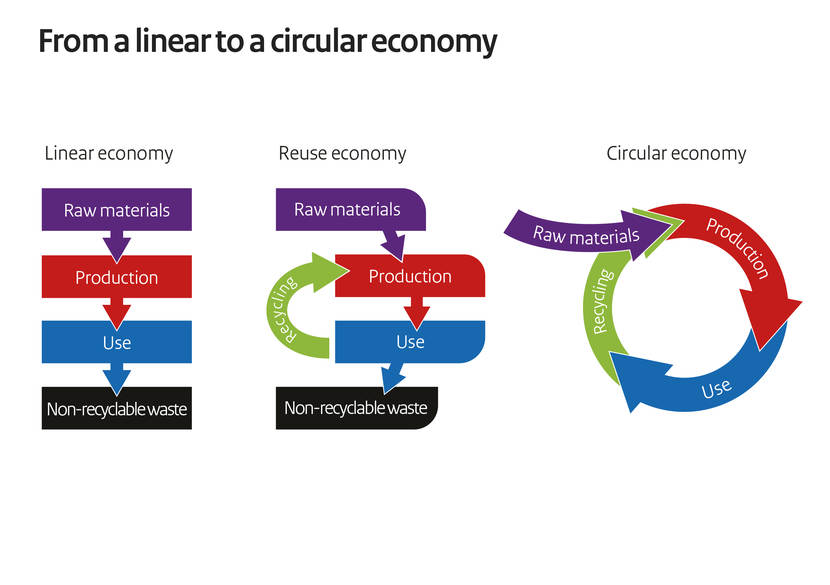
\includegraphics[width=0.7\linewidth]{Images/from-linear-to-a-circulair-economy.jpg}
        \caption{From a linear to a circular economy \cite{GovernmentoftheNetherlands2021}.}
    \label{fig:From a linear to a circular economy.}
\end{figure}
